\section{Markovketten und Markovmodelle}

\begin{definition}[Markov-Eigenschaft]

    Man sagt ein stochastischer Prozess $\{X_t\}_{t \in T}$ besitzt die \textbf{Markov-Eigenschaft}, wenn der Zustand des nächsten Zeitpunktes $t +1$ einzig und allein vom Zustand im gegenwärtigen Zeitpunkt $t$ abhängt.
    \begin{equation}
        P(X_{t+1}=i_{t+1} \mid X_{t} = i_{t}, \dots, X_2=i_2, X_1=i_1) = P(X_{t+1}=i_{t+1} \mid X_{t} = i_{t})
    \end{equation}
    Für alle $t \in T$ und alle $i_k \in S$ unter der Vorraussetzung, dass alle bedingten Wahrscheinlichkeiten Wohldefiniert sind, also $P(X_{t} = i_{t}, \dots, X_2=i_2, X_1=i_1) > 0$.
\end{definition}

\begin{definition}[Markovkette]

    Eine Markovkette ist gegeben durch einen stochastischen Prozess $\{X_t\}_{t \in T}$, welcher Werte aus einer Menge an Zuständen $S = \{s_1, s_2, \dots, s_n\}$ annehmen kann und die Markov-Eigneschaft erfüllt. Solch ein Markovprozess wird beschrieben durch zwei Variablen. Einen \textbf{Startwahrscheinlichkeitsvektor} $\pi$ mit Länge $n$ und eine \textbf{Transitionsmatrix} $A$ mit Dimension $n \times n$, wobei $n$ die Anzahl der Zustände $S$ ist. $\pi_i$ gibt die Wahrscheinlichkeit an, in Zustand $s_i$ zu starten. Also die Wahrscheinlichkeit, dass sich der Prozess in Zeitpunkt $t=0$ in Zustand $s_i$ befindet.
    \begin{equation}
        \pi_i = P(X_0 = s_i)
    \end{equation}
    Die Transitionsmatrix $A$ beschreibt die bedingten Wahrscheinlichkeiten, mit denen ein Zustandsübergang geschieht. $a_i(j)$ ist die Wahrscheinlichkeit dass sich der Prozess in Zeitpunkt $t+1$ in Zustand $s_j$ befindet, unter der Bedingung das er sich in Zeitpunk $t$ in Zustand $s_i$ befindet.
    \begin{equation}
        a_{ij} = P(X_{t+1} = s_j \mid X_t = s_i)
    \end{equation}
\end{definition}

Eine Markovkette ist \textbf{zeithomogen} wenn die Transitionswahrscheinlichkeiten $a_{ij}$ unabhängig von der Zeit $t$ sind \cite{HmmIntroduction}.
\begin{align}
    a_{ij} = P(X_{t+1} = s_j \mid X_t = s_i) = P(X_{t} = s_j \mid X_{t-1} = s_i) && 
\end{align}
In dieser Arbeit werden ausschließlich zeithomogene Markovketten betrachtet.

Das Ereignis in irgendeinem Zustand zu starten, so wie das Ereignis von einem gegebenen Zustand in irgendeinen anderen Zustand zu wechseln sind sichere Ereignisse. Somit gelten die Bedingungen, dass die Werte des Startwahrscheinlichkeitsvektors $\pi$ und die Werte der ausgehenden Transitionen für jeden Zustand $A_i$ in Summe jeweils 1 ergeben müssen. Diese Bedingung nennt man \textbf{Reihenstochastizität}
\begin{align}
    \sum_{i = 0}^{N} \pi_i = 1 && \sum_{j = 0}^{N} a_{ij} = 1
\end{align}

Als Beispiel für eine zeitdiskrete homogene Markovkette werden wir die durchschnittliche jährliche Temperatur modellieren. Seien die Zustände des Modells gegeben durch $S=\{H, K\}$, wobei $H$ für heiß und $K$ für kalt steht. Der Startvektor $\pi$ und die Transitionsmatrix $A$ seien gegeben durch
\begin{align}
    \pi = (0.7, 0.3) && 
    A = 
    \begin{bmatrix}
        0.8 & 0.2 \\
        0.4 & 0.6 \\
    \end{bmatrix}
\end{align}

Wir können diese Markovkette anschaulich als gerichteten Transitionsgraphen representieren.

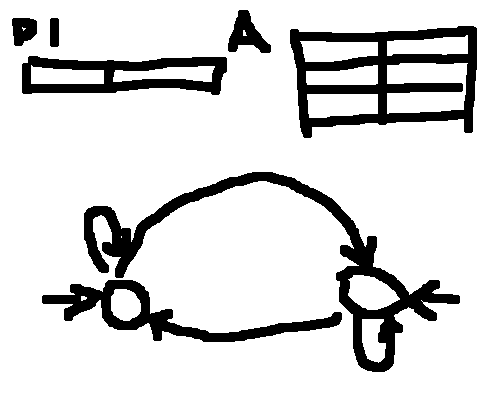
\includegraphics[scale=1.0]{images/Markov_Chain_Example.png}

Mit unserem Temperaturmodell können wir nun zum Beispiel berechnen, was die Wahrscheinlichkeit ist die Temperaturabfolge $O = \{H, K, K, H, H\}$ zu beobachten.
\begin{align*}
    P(O) & = P(O_1 = H) \cdot P(O_2 = K \mid O_1 = H) \cdot P(O_3 = K \mid O_2 = K) \\
    & \cdot P(O_4=H \mid O_3 = K) \cdot P(O_5 = H \mid O_4 = H) \\
    & = \pi_1 \cdot a_{12} \cdot a_{22} \cdot a_{21} \cdot a_{11} \\
    & = 0.7 \cdot 0.2 \cdot 0.6 \cdot 0.4 \cdot 0.8 = 0.02688
\end{align*}

Eine Markovkette gibt uns also die möglichkeit probabilistische Systeme, in denen wir die Zustände und die Zuständsübergänge direkt beobachten können zu modellieren.

\subsection{Hidden Markov Modelle (HMMs)}
Bei einem Hidden Markov Modell ist die Observationssequenz nicht identisch zur Zustandssequenz, sondern die Observationssymbole sind das Ergebnis einer stochastischen Funktion der Zustände. Die Zustände selbst, so wie die Zustandsübergänge können wir \textit{nicht beobachten} denn die Zustände sind ,,hidden". Ein HMM besteht also aus zwei stochastischen Prozessen. Ein versteckter Prozess, der die Transitionen in Abhängigkeit des vorherigen Zustandes bestimmt und ein zweiter Prozess, der die Observationssymbole in Abhängigkeit des gegenwärtigen Zustandes bestimmt.
Formal definieren wir ein Hidden Markov Modell wie folgt.
\begin{definition}[Hidden Markov Modell]
    Ein Hidden Markov Modell ist definiert durch den Startwahrscheinlichkeitsvektor $\pi$ und die Transitionsmatrix $A$ einer Markovkette und einer zusätzlichen \textbf{Emissionsmatrix} $B=\{b_j(k)\}$ mit Dimension $N \times M$ wobei $N$ die Anzahl der Zustände der Markovkette und $M$ die Anzahl der möglichen Observationssymbole ist. Die Emissionsmatrix $B$ gibt die Wahrscheinlichkeit eines Observationssymbols $v_k$ unter der Bedingung, dass sich der Prozess im gegenwärtigen Zeitpunkt $t$ in Zustand $s_j$ befindet an.
    \begin{align}
        b_j(k) = P(O_t = v_k \mid q_t = S_j) && 1 \leq j \leq N && 1 \leq k \leq M
    \end{align}
\end{definition}
Wie ein solches HMM nun eine Observationssequenz $O$ von Länge $T$ erzeugen kann möchte ich durch folgendes Gedankenexperiment verdeutlichen.
Stellen wir uns einen Raum vor, in dem $N$ Urnen stehen. Die Urnen enthalten Kugel aus $M$ verschiedenen Farben, wobei die Urnen verschiedene Verteilungen dieser Farben enthalten können. In dem Raum befindet sich eine Person welche nun insgesamt $T$ Kugeln aus den Urnen ziehen und zurücklegen wird, wobei sie sich abhängig von einem Zufallsprozess von einer Urne zur nächsten bewegt. Wir können in diesen Raum nicht hineinsehen und somit nicht beobachten aus welcher Urne ein Kugel gezogen wurde. Wir kennen nur die Observationssequenz, also die Abfolge der Farben der gezogenen Kugeln. Um ethische Bedenken über dieses Gedankenexperiment zu minimieren sei angemerkt, dass der Raum klimatisiert ist und der Person Kakao und Kekse zur Verfügung stehen.
\begin{itemize}
    \item Zunächst wird die initiale Urne anhand des Startwahrscheinlichkeitsvektor $\pi$ ausgewählt.
    \item Dann zieht die Person eine Kugel aus der Urne, notiert deren Farbe als $O_1$ und legt die Kugel zurück.
    \item Danach wird eine neue Urne $q_2 = S_j$ mit Wahrscheinlichkeit $a_{ij} = P(q_2 = S_j \mid q_1 = S_1)$ gewählt. Aus dieser neuen Urne wird die nächste Kugel $O_2$ der Farbe $v_k$ mit Wahrscheinlichkeit $b_j(k)$ gezogen.
\end{itemize}
Diese Prozedur wird so oft wiederholt bis der Zeitpunkt $t=T$ erreicht ist. Wir erhalten somit eine Observationssequenz von Farben $O= \{O_1, O_2, \dots, O_T \}$.
Abbildung \ref{fig:urn_ball_model} zeigt eine Visualisierung dieses Gedankenexperiments für $N=3$

\begin{figure}[h!]
    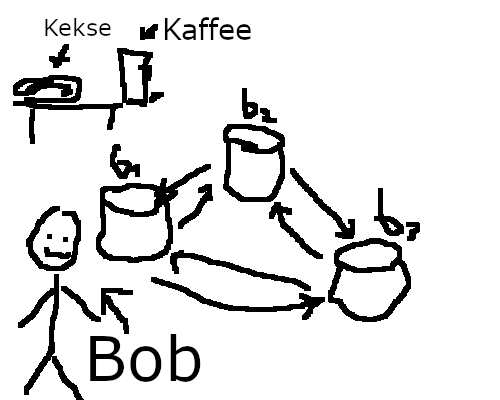
\includegraphics[scale=1.0]{images/Ball_Urn_Model.png}
    \caption{Urn Ball Model}
    \label{fig:urn_ball_model}
\end{figure}